\documentclass[border=10pt]{standalone}
\usepackage{tikz}
\usetikzlibrary{3d,calc}

\begin{document}
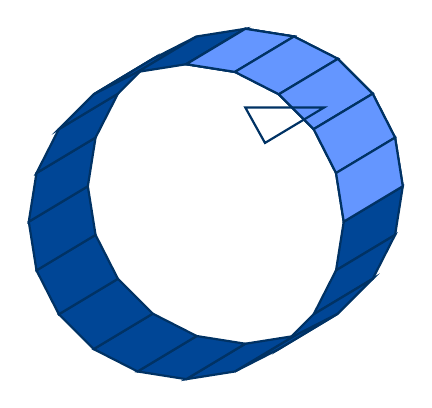
\begin{tikzpicture}[x={(1cm,0cm)},y={(0cm,1cm)},z={(-0.5cm,-0.3cm)}]

% Define parameters
\def\n{20} % number of segments
\def\r{2}  % radius of the curve
\def\h{1.5} % height of the ribbon
\def\w{0.1} % width of each segment

% Define color gradient
\definecolor{darkblue}{RGB}{0,50,100}
\definecolor{mediumblue}{RGB}{0,70,150}
\definecolor{lightblue}{RGB}{100,150,255}

% Draw the ribbon
\foreach \i in {0,...,\n} {
    \pgfmathsetmacro{\angle}{90 - \i * 360 / \n}
    \pgfmathsetmacro{\x}{\r * cos(\angle)}
    \pgfmathsetmacro{\y}{\r * sin(\angle)}
    \pgfmathsetmacro{\nextangle}{90 - (\i+1) * 360 / \n}
    \pgfmathsetmacro{\nx}{\r * cos(\nextangle)}
    \pgfmathsetmacro{\ny}{\r * sin(\nextangle)}
    
    % Calculate color based on position
    \pgfmathsetmacro{\shade}{\i / \n * 100}
    \ifnum\i<\n
        \ifnum\i<5
            \definecolor{currentcolor}{RGB}{100,150,255} % light blue for inner part
        \else
            \definecolor{currentcolor}{RGB}{0,70,150} % medium blue for main part
        \fi
    \else
        \definecolor{currentcolor}{RGB}{0,50,100} % dark blue for end
    \fi
    
    % Draw the segment
    \draw[fill=currentcolor, draw=darkblue, thick] 
        (\x,\y,0) -- (\x,\y,\h) -- (\nx,\ny,\h) -- (\nx,\ny,0) -- cycle;
}

% Add inner cutout (notch)
\foreach \i in {0,...,4} {
    \pgfmathsetmacro{\angle}{90 - \i * 360 / \n}
    \pgfmathsetmacro{\x}{\r * cos(\angle)}
    \pgfmathsetmacro{\y}{\r * sin(\angle)}
    \pgfmathsetmacro{\nextangle}{90 - (\i+1) * 360 / \n}
    \pgfmathsetmacro{\nx}{\r * cos(\nextangle)}
    \pgfmathsetmacro{\ny}{\r * sin(\nextangle)}
    
    \draw[fill=lightblue, draw=darkblue, thick] 
        (\x,\y,0) -- (\x,\y,\h) -- (\nx,\ny,\h) -- (\nx,\ny,0) -- cycle;
}

% Add outline for depth
\draw[thick, darkblue] 
    plot[domain=0:1, samples=50, smooth] 
    (\x,\y,0) -- (\nx,\ny,0) -- (\nx,\ny,\h) -- (\x,\y,\h) -- cycle;

\end{tikzpicture}
\end{document}